
\section{Results}
\label{sec:results}

Our final results and code are in \texttt{b6\_model\_final.ipynb} and \texttt{huntington\_model\_final.ipynb}. We evaluated the quality of fitting across all our models using the R-squared value and root mean square error (RMSE) analyses.
\subsection{Beach 6}
For the Beach 6 dataset, we found that all four models we generated have higher R-squared values while maintaining lower RMSE values than the published model (Figure \ref{fig:b6}). This result surprised us, although we realized that our fine-tuning of coefficients using cross-validation and grid search could contribute to better performance. Having lower scores on training data, yet higher scores on testing data, indicates the absence of overfitting in our models.\\
Looking into each model for the Beach 6 dataset, we found that the performance of Ridge and PolyRidge was the same. We then plotted the graphs of actual values versus predicted values for both models (Figure \ref{fig:b6ridge}, \ref{fig:b6poly}). We observed a consistent pattern of prediction versus actuality. This was due to the preference of hyper-parameter dimension by the grid search. We found that in our code, grid search selected degree = 1, which reduces to a linear model, leading to the identical performance by Ridge and PolyRidge.\\
The result of our differential analysis suggested that the prediction could be strongly affected by the hyperparameter \texttt{BIRDS\_NUM}. The huge swing between discrete numbers could potentially contribute huge variance during prediction. The p-value of the \texttt{BIRDS\_NUM} coefficient also suggested that, compared to other coefficients, it is more prone to generate variant results.
\subsection{Huntington}
For the Huntington dataset, our models generally performed as well as the published one (Figure \ref{fig:hunt}). The PolyRidge model wins with an exceptional $0.56590$ R-squared value and $0.4336$ RMSE. It indicates that the connections between hyperparameters are of significance to the prediction of \textit{E. coli} concentration in Huntington.\\
We also plotted the predicted versus actual values for the PolyRidge and Ridge models to see the differences. We observed that although the patterns are consistent when on the lower end ($\log_{10}$ \textit{E. coli} concentration $\leq 2.0$), the PolyRidge model produces more converged data on the higher end ($\log_{10}$ \textit{E. coli} concentration $> 2.0$). This suggested that in order to predict higher values better, a higher degree of hyperparameters is necessary.
The differential analysis unravels the effect of the hyperparameter \texttt{WaveHt\_Ft} on the prediction. We found multiple zero values among the top ten outliers. Since the model is using polynomial regression, any combination of hyperparameters associated with \texttt{WaveHt\_Ft} would be zero. This could cause a major fluctuation between the predicted and actual values.

\begin{figure}
    \centering
    \resizebox{0.47\textwidth}{!}{
        \begin{tabular}{|c|c|c|c|c|}
             \hline
             Model & Train $R^2$ Mean & Train RMSE Mean & Test $R^2$ & Test RMSE\\[3pt]
             \hline
             Published & N/A & N/A & $0.47697$ & $0.4841$\\[3pt]
             \hline
             Ridge & $0.42921$ & $0.5032$ & $0.48872$ & $0.4431$\\[3pt]
             \hline
             PolyRidge & $0.42921$ & $0.5032$ & $0.48872$ & $0.4431$\\[3pt]
             \hline
             SGD & $0.42833$ & $0.5029$ & $0.48851$ & $0.4432$\\[3pt]
             \hline
             LASSO & $0.42817$ & $0.5033$ & $0.48912$ & $0.4429$\\[3pt]
             \hline

        \end{tabular}
        }
    \caption{Model performance on the Beach 6 dataset}
    \label{fig:b6}
\end{figure}

\begin{figure}
    \centering
    \resizebox{0.47\textwidth}{!}{
        \begin{tabular}{|c|c|c|c|c|}
             \hline
             Model & Train $R^2$ Mean & Train RMSE Mean & Test $R^2$ & Test RMSE\\[3pt]
             \hline
             Published & N/A & N/A & $0.54985$ & $0.4432$\\[3pt]
             \hline
             PolyRidge & $0.54241$ & $0.4423$ & $0.56590$ & $0.4336$\\[3pt]
             \hline
             Ridge & $0.53913$ & $0.4438$ & $0.54807$ & $0.4424$\\[3pt]
             \hline
             LASSO & $0.53904$ & $0.4438$ & $0.54774$ & $0.4426$\\[3pt]
             \hline
             SGD & $0.53856$ & $0.4440$ & $0.54826$ & $0.4423$\\[3pt]
             \hline

        \end{tabular}
        }
    \caption{Model performance on the Huntington dataset}
    \label{fig:hunt}
\end{figure}

\begin{figure}
    \centering
    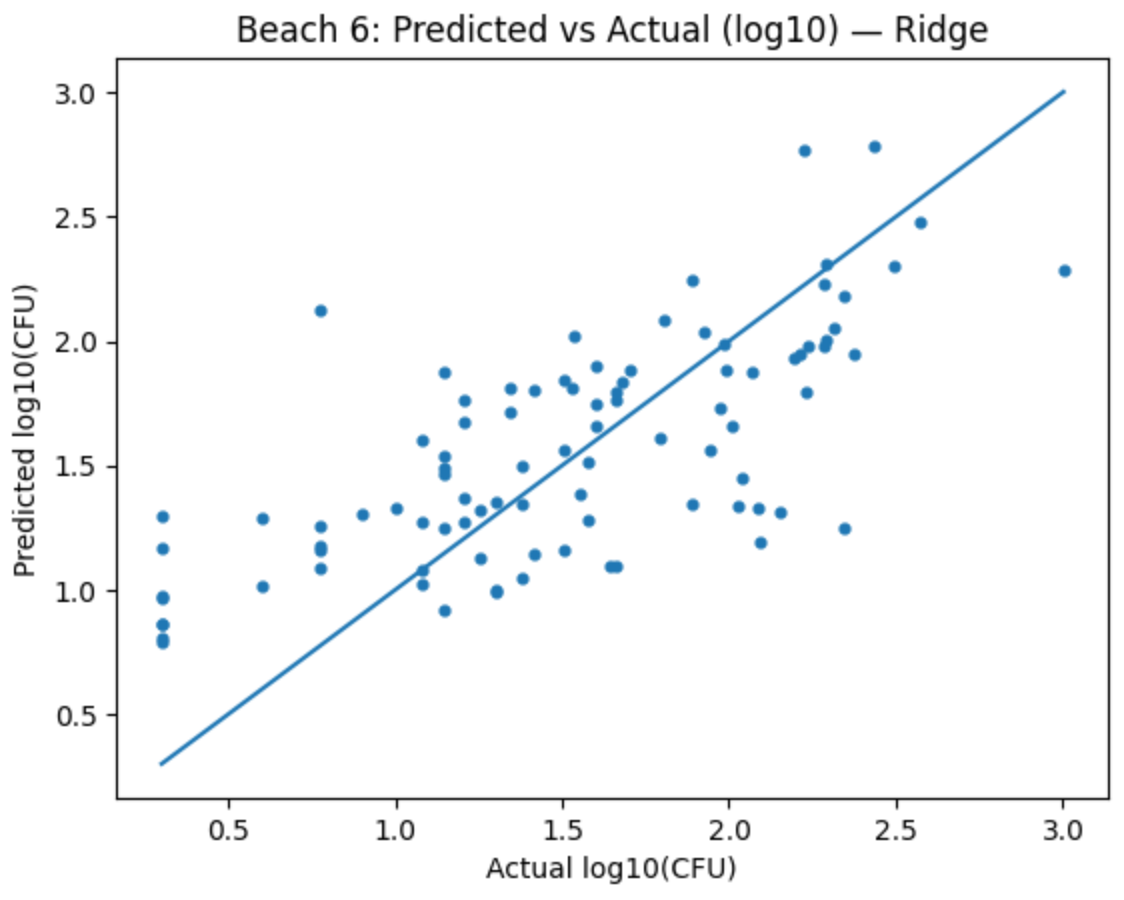
\includegraphics[width=0.86\linewidth]{figs/b6_ridge.png}
    \caption{Predicted versus actual values for Beach 6 dataset using Ridge linear regression model.}
    \label{fig:b6ridge}
\end{figure}

\begin{figure}
    \centering
    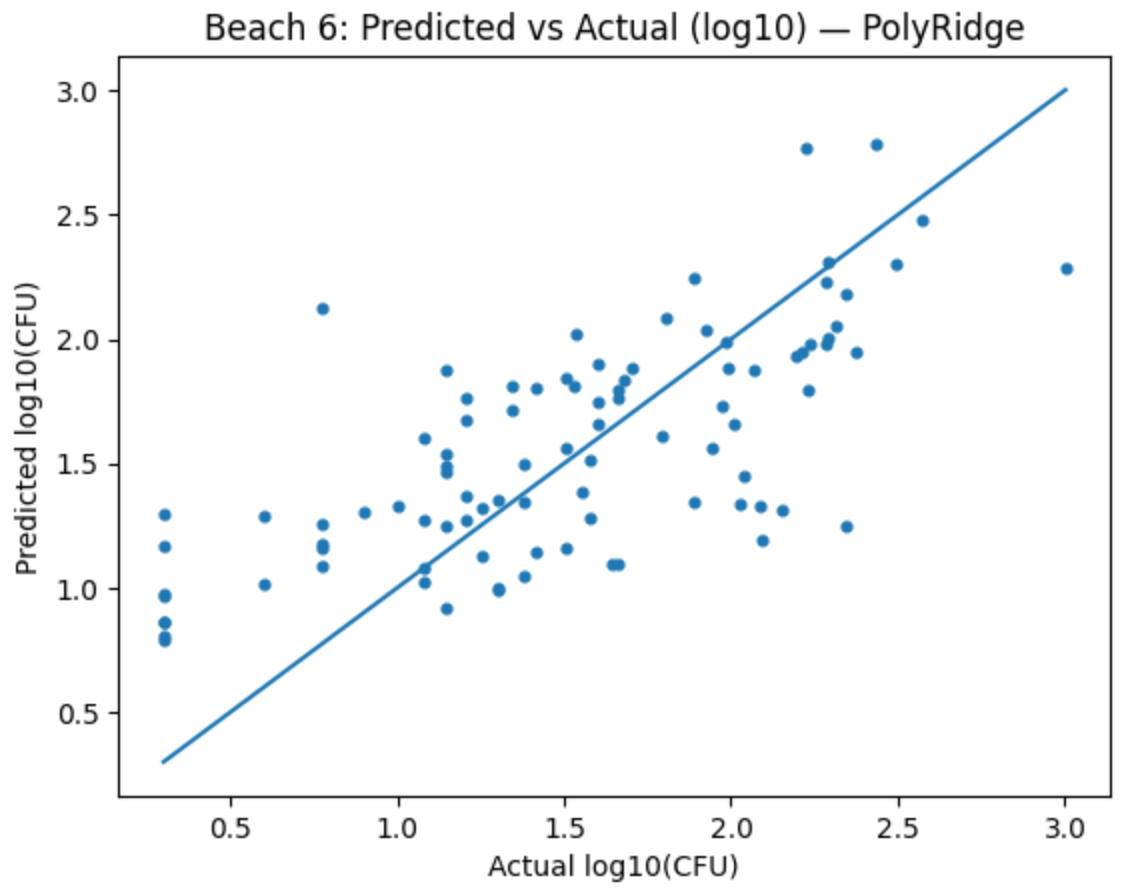
\includegraphics[width=0.86\linewidth]{figs/b6_poly.png}
    \caption{Predicted versus actual values for Beach 6 dataset using PolyRidge linear regression model.}
    \label{fig:b6poly}
\end{figure}

\begin{figure}
    \centering
    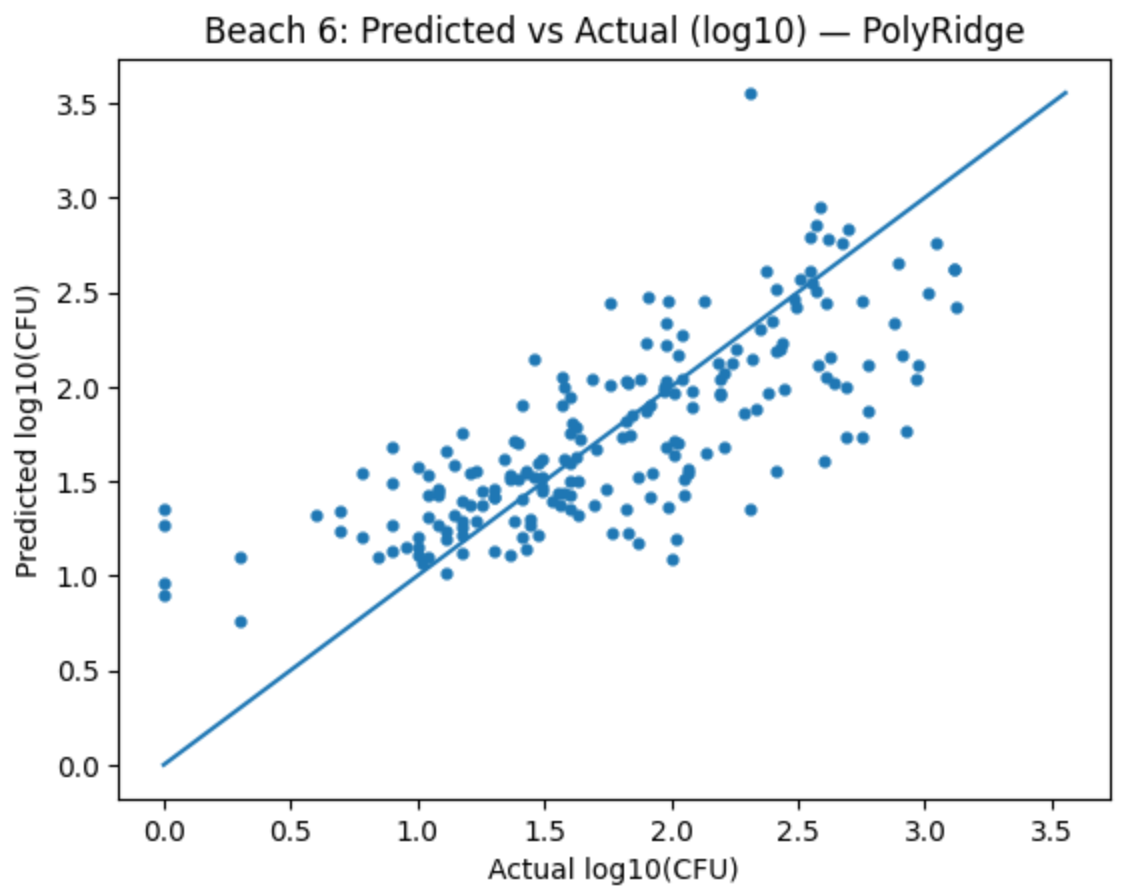
\includegraphics[width=0.86\linewidth]{figs/hunt_poly.png}
    \caption{Predicted versus actual values for Huntington dataset using PolyRidge linear regression model.}
    \label{fig:huntPoly}
\end{figure}

\begin{figure}
    \centering
    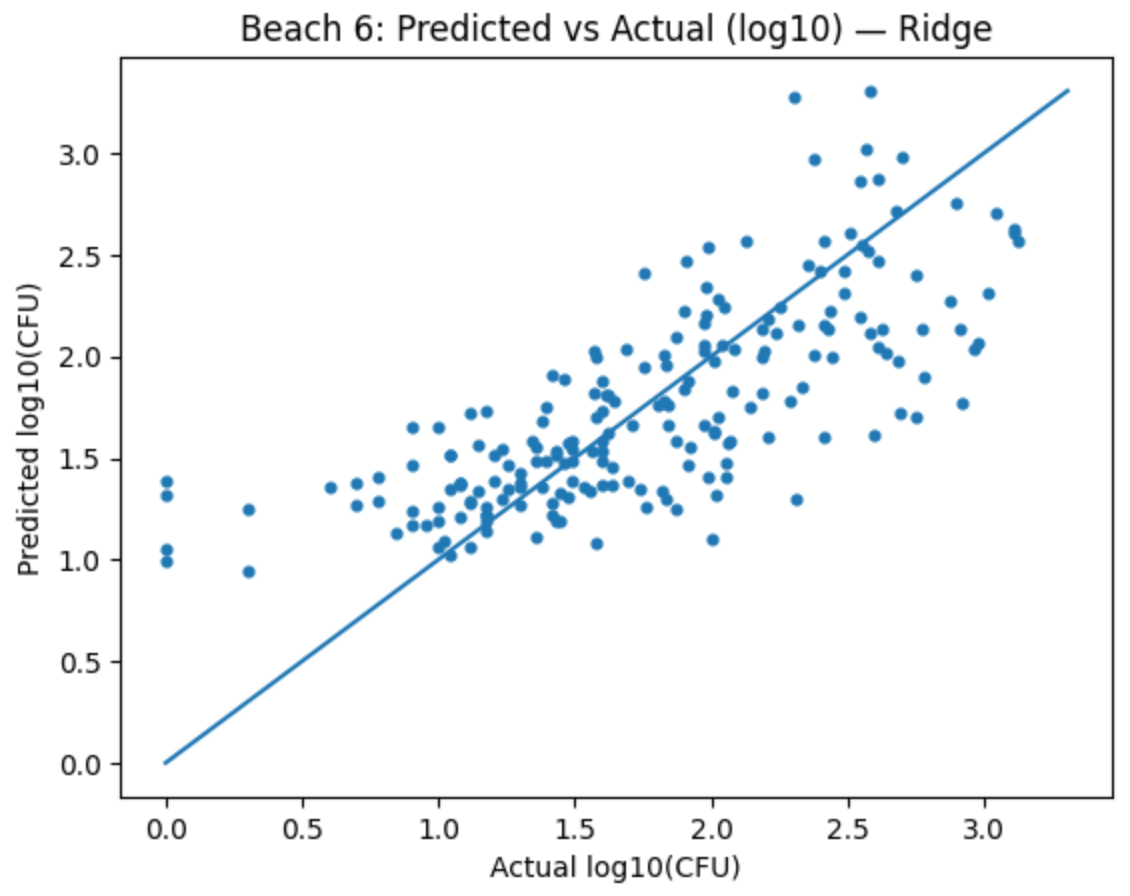
\includegraphics[width=0.86\linewidth]{figs/hunt_ridge.png}
    \caption{Predicted versus actual values for Huntington dataset using Ridge linear regression model.}
    \label{fig:huntRidge}
\end{figure}
